
Un trabajo desarrollado por la Universidad de Tsukuba en
 Jap\'on\cite{Nakano2006}, tiene por objetivo el crear un oponente virtual
 al nivel de un oponente humano que represente un reto para el jugador. Para
 lograr esto se crearon perfiles con las estrategias de los jugadores y
 posteriormente se reproducen en otra partida, en la figura~\ref{fig:imitat}
 se muestra el entorno del juego.


\begin{figure}[h]
\centering
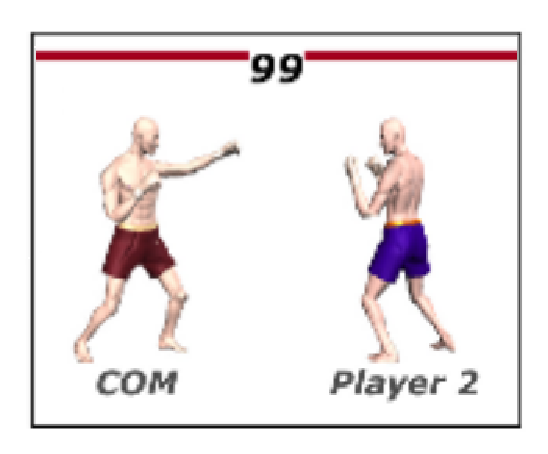
\includegraphics[width=0.5\columnwidth]{chap2/Imagenes/Imitating.eps}
\caption{Ambiente del juego de acci\'on.}
\label{fig:imitat}
\end{figure}